\documentclass[10pt]{article}
\usepackage{../../local}


\newcommand{\classcode}{Physics 112}
\newcommand{\classname}{Introduction to Statistical Mechanics}
\renewcommand{\maketitle}{%
\hrule height4pt
\large{Eric Du \hfill \classcode}
\newline
\large{HW 05} \Large{\hfill \classname \hfill} \large{\today}
\hrule height4pt \vskip .7em
\normalsize
}
\linespread{1.1}
\begin{document}
	\maketitle
	\section*{Schroeder 4.3}

	A power plant produces 1 GW of electricity, at an efficiency of 40\% (typical of today's coal-fired
	plants). 

	\begin{enumerate}[label=\alph*)]
		\item At what rate does this plant expel waste heat into its environment?

			\begin{solution}
				To calculate the rate, consider what occurs during one second of operation. The efficiency 
				is given by 
				\[
					\epsilon = 1 - \frac{Q_c}{Q_h}
				\] 
				Therefore, 
				\[
					\frac{Q_c}{Q_h} = 1 - \epsilon = 0.6
				\] 
				therefore, $Q_c = 0.6 Q_h$. Further, we have 
				\[
					\frac{W}{Q_h} = \frac{1 \text{GJ}}{Q_h} = 0.4 \implies Q_h = 2.5 \text{ GJ}
				\] 
				Finally, putting it all together, we have:
				\[
					Q_c = 0.6 Q_h = (0.6)(2.5 \text{ GJ}) = 1.5 \text{ GJ}
				\] 
				We took this over 1 second, so the rate of heat expulsion is 1.5 GW.
			\end{solution}
		\item Assume first that the cold reservoir for this plant is a river whose flow rate is 100 
			$\mathrm{m^3/s}$. By how much will the temperature of the river increase?

			\begin{solution}
				Again, consider a unit time of 1 second. There are $100 \mathrm{m^3}$ of water, during which 
				1.5 GJ of energy is being dumped into it. From the back of the book, we have $C_P = 75.29$ J/K
				at a volume of $18.068 \mathrm{\ cm^3}$, so this corresponds to $C_P = 4.18 \mathrm{\ J/cm^3 K}$.
				We want this value in units of $\mathrm{J/m^3 K}$ since our heat is in units of cubic meters, 
				so therefore this corresponds to $C_P = 4.18 \times 10^6 \mathrm{\ J/m^3 K}$. Now, 
				we divide:
				\[
					Q_c = (C_P V) \Delta T \implies \Delta T = \frac{Q_c}{C_P V} =
					\frac{1.5 \times 10^{9}}{(4.18 \times 10^6
					\mathrm{\ J/m^3 K })(100 \mathrm{\ m^3})} = 3.58 \  \mathrm{K}
				\] 
				So we see that the water warms up by 3.58 K. 
			\end{solution}
		\item To avoid this ``thermal pollution" of the river, the plant could instead be cooled by 
			evaporation of water. (This is more expensive, but in some areas it is environmentally preferable.) 
			At what rate must the water evaporate? What fraction of the river must be evaporated?

			\begin{solution}
				We follow the outline in the problem statement, by considering $\Delta H$. Specifically, 
				let 
				\[
					\Delta H_f = H_{\ch{H2O}, g} - H_{\ch{H2O}, l} = 44.01 \ \mathrm{kJ / mol}
				\] 
				This is the energy required to evaporate one mole of water, according to the table. Therefore, 
				the required volume is:
				\[
					V_{\text{req}} = \frac{Q}{\Delta H_f} = \frac{1.5 \times 10^6 \ \text{kJ}}{44.01 \text{kJ / mol}} \cdot 18.068 \ \mathrm{cm^3/mol} = 615,815 \ \mathrm{cm^3}
				\] 
				Converting this to cubic meters, this comes out to approximately $0.6 \ \mathrm{m^3}$ per 
				second, so about 0.6\% of the river. 
			\end{solution}
	\end{enumerate}
\pagebreak	
	\section*{Problem 2}
	An ideal gas with $f$ degrees of freedom per molecule undergoes the cyclic process shown below. Step 
	$2 \to 3$ is adiabatic.

	\begin{center}
		\begin{tikzpicture}[scale=0.8]
			\draw[thick] (0, 0) -- (5, 0) node[right] {$V$};
			\draw[thick] (0, 0) -- (0, 5) node[above] {$P$};
			\draw[postaction={on each segment={mid arrow=black}}] (1, 1) node[below left] {1} -- (1, 3) node[above left] {2} to [style=bend right, looseness=0.5] 
				(4.5, 1) node[right] {3}  -- cycle;
			\draw[dashed] (1, 0) node[below] {$V_1$} -- (1, 1);
			\draw[dashed] (0, 3) node[left] {$P_2$} -- (1, 3); 
			\draw[dashed] (0, 1) node[left] {$P_1$} -- (1, 1);
			\draw[dashed] (4.5, 0) node[below] {$V_2$} -- (4.5, 1);
		\end{tikzpicture}
	\end{center}
	\begin{enumerate}[label=\alph*)]
		\item For each of the steps $1 \to 2$, $2 \to 3$, $3 \to 1$, compute $\Delta U, Q, W$ with 
			$\Delta U = Q + W$. Express your answers in terms of $V_1, V_2, P_1, f, \gamma = (f + 2) / f$. 
			Summarize the final answer into a 3-row table with columns $\Delta U, Q, W$.

			\begin{solution}
				Step $1 \to 2$ is held at constant volume, so $W = -P \Delta V = 0$. Therefore, $\Delta U = 
				Q = \Delta(\frac{f}{2}PV)$, so we have:
				\[
				\Delta U = \frac{f}{2}V_1(P_2 - P_1) = Q
				\] 
				Step $2 \to 3$ is adiabatic, so $Q = 0$, and $\Delta U = W$. In order to calculate the 
				work done, we use the integral form of the work:
				\[
					W = -\int_{V_1}^{V_2} P(V) dV
				\] 
				Since this is an adiabat, then we know that $PV^\gamma = \text{const.}$, so we have 
				$P(V) = \frac{c}{V^\gamma}$. Now we can integrate:
				\begin{align*}
					W &=  -\int_{V_1}^{V_2} \frac{c}{V^\gamma} dV \\
					  &= -\left[ \frac{c}{1-\gamma}V^{1 - \gamma} \right]_{V_1}^{V_2} \\
					  &= \frac{c}{1 - \gamma}\left[V_1^{1 - \gamma} - V_2^{1 - \gamma}\right] \\
					  &= \frac{c}{1 - \gamma}V_1^{1 - \gamma } \left[ 1 - \left( \frac{V_2}{V_1} \right)^{1 - \gamma} \right] \\
					  &= \frac{P_1V_1}{1 - \gamma}\left( \frac{V_2}{V_1} \right)^{1 - \gamma} 
					  \left[ 1 - \left( \frac{V_2}{V_1} \right)^{1 - \gamma} \right] = \Delta U
				\end{align*}
				Finally, for step $3 \to 1$, we're at constant pressure, so $W = -P_1\Delta V = 
				-P_1(V_1 - V_2)$. As for $Q$:
				\begin{align*}
					Q &= \Delta U - W\\
					&= \frac{f}{2}P_1(V_1 - V_2) + P_1(V_1 - V_2) \\
					&= P_1(V_1 - V_2)\left( \frac{f}{2}+1 \right)  
				\end{align*}
			\end{solution}
		\item Viewed as an engine, what is the thermodynamic efficiency $\epsilon$ of the process? (I apologize, 
			the expression isn't very beautiful). Your final answer should depend only on $f, \gamma
			V_2 / V_1$. Using $f = 5$, produce a plot of $\epsilon(V_2/V_1)$.

			\begin{solution}
				The efficiency is calculated using $\epsilon = 1 - \frac{Q_c}{Q_h}$, so we need to identify 
				which process does heat enter and leave the system. Clearly, since the heat from $1 \to 2$ 
				is positive and $3 \to 1$ is negative, then $Q_h$ is the heat from $1 \to 2$ and $Q_c$ is 
				the heat from $3 \to 1$. In order for the efficiency to be less than 1, we need to flip $Q_c$ 
				so that it's positive. In the end, the efficiency is:
				\begin{align*}
					\epsilon &= 1 - \frac{P_1(V_2 - V_1)(\frac{f}{2} + 1)}{\frac{f}{2}P_1V_1\left[
					\left( \frac{V_2}{V_1} \right) ^\gamma - 1\right]}\\
							 &= 1 - \frac{\left( \frac{V_2}{V_1} - 1 \right) (f + 2)}{f\left[ \left( \frac{V_2}{V_1} \right) ^\gamma - 1 \right] }\\
							 &= 1 - \frac{\gamma\left( \frac{V_2}{V_1}-1 \right) }{\left( \frac{V_2}{V_1} \right) ^\gamma - 1} 
				\end{align*}
				A plot of this is shown below, for $f = 5$:
				\begin{center}
					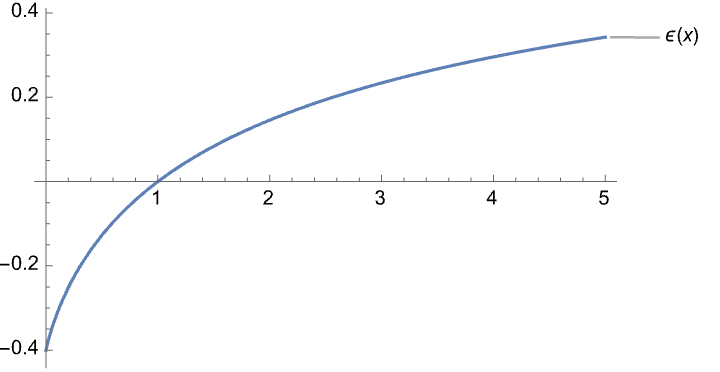
\includegraphics[scale=0.7]{e.png}
				\end{center}
				Note that the efficiency is negative when $\frac{V_2}{V_1}< 1$, which makes sense since 
				that means that $V_2 < V_1$, so this regime doesn't model our system at all. Therefore 
				in some sense, we only care about the regime where $\frac{V_2}{V_1}> 1$, where 
				our efficiency is positive. 
			\end{solution}
		\item In order to compare with Carnot efficiency, find an expression for the hottest $T_h$ and 
			coldest $T_c$ temperatures of the gas during the cycle. Compute the resulting Carnot efficiency 
			$\epsilon_C$ for reservoirs at these temperatures. In order to compare with part b, plot 
			$\epsilon_C(V_2 / V_1)$ for $f = 5$ on the same plot.

			\begin{solution}
				Since $PV = NkT$ then $T = \frac{PV}{Nk}$, hence $T \propto PV$. Therefore, we are looking
				for the values that maximize and minimize $PV$. For the minimum, this is fairly obvious:
				point 1 should be the one we choose. For the maximum, we need to compare the temperature 
				at points 2 and 3. Looking at point 2 more closely, we can use $PV^\gamma$ to compare with 
				point 3:
				\begin{align*}
					P_2V_1 &= P_1\left( \frac{V_2}{V_1} \right)^\gamma V_1 \\
						   &= P_1V_2 \cdot V_2^{\gamma - 1} V_1^{1 - \gamma} \\
						   &= P_1V_2\left( \frac{V_2}{V_1} \right)^{\gamma - 1} > P_1V_2
				\end{align*}
				so we conclude that point 2 is $T_h$. Thus, we have:
				\begin{align*}
					\epsilon_C &= 1 - \frac{T_c}{T_h}\\
					&= 1 - \frac{P_1}{P_1\left( \frac{V_2}{V_1} \right)^\gamma} \\
					&=  1 - \left( \frac{V_1}{V_2}\right)^\gamma \\
					&= 1 - \left(\frac{V_2}{V_1}\right)^{-\gamma}
				\end{align*}
				Plotting both of these below:
				\begin{center}
					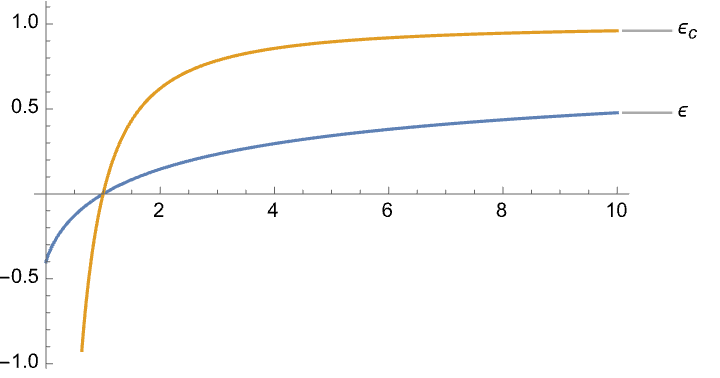
\includegraphics[scale=0.7]{ec.png}
				\end{center}
				Again like the previous plot, we only care about the regime where $\frac{V_2}{V_1} > 1$. One 
				thing to note is that when $V_2 \gg V_1$, that both efficiencies approach 1, However, 
				$\epsilon$ approaches this limit much more slowly than $\epsilon_C$.  
			\end{solution}
		\item Viewed as a heat pump, what is the thermodynamic efficiency of the process?

			\begin{solution}
				A heat pump is the same thing as a refrigerator, except we have a different interpretation 
				of what is considered a ``benefit'' in our system. In this case, the ``benefit'' is $Q_h$,
				and the cost is still $W$, so we have:
				\[
					\mathrm{COP} = \frac{Q_h}{W}
				\] 
				Note that our expression for $\epsilon$ in part (b) is the inverse of this, so we 
				conclude:
				\begin{align*}
					\mathrm{COP} &= \frac{1}{\epsilon} \\
								 &= \left[ 1 - \frac{\gamma\left( \frac{V_2}{V_1} - 1 \right) }{\left( \frac{V_2}{V_1} \right)^\gamma - 1} \right]^{-1}\\
								 &= \left[ \frac{\left( \frac{V_2}{V_1} \right)^\gamma - \gamma\left( \frac{V_2}{V_1}-1 \right) - 1 }{\left( \frac{V_2}{V_1} \right)^\gamma - 1}\right]^{-1}  \\
					&= \frac{\left( \frac{V_2}{V_1} \right)^\gamma - 1}{
					\left( \frac{V_2}{V_1} \right)^\gamma -\gamma \left( \frac{V_2}{V_1} -1\right)-1 }\\
				\end{align*} 
				Unfortunately this expression is also not very clean, but there's nothing much I can do about it.
			\end{solution}
	\end{enumerate}

	\pagebreak

	\section*{Schroeder 4.6}
	To get more than an infinitesimal amount of power out of a Carnot engine, we would have to keep 
	the temperature of its working substance below that of the hot reservoir and above that of the cold 
	reservoir by non-infinitesimal amounts. Consider, then, a Carnot cycle in which the working substance 
	is at temperature $T_{hw}$ as it absorbs heat from the hot reservoir, and at temperature $T_{cw}$ as 
	it expels heat to the cold reservoir. Under most circumstances the rates of heat transfer 
	will be directly proportional to the temperature differences:
	\[
		\frac{Q_h}{\Delta t} = K(T_h - T_{hw}) \hspace{1.5cm} \text{and}\hspace{1.5cm} \frac{Q_c}{\Delta t} = K(T_{cw} - T_c)
	\]   
	I've assumed here for simplicity that the constants of proportionality ($K$) are the same for both 
	of these processes. Let us also assume that both processes take the same amount of time, so the 
	$\Delta t$'s are the same in both of these equations.
	\begin{enumerate}[label=\alph*)]
		\item Assuming that no new entropy is created during the cycle except during the two heat transfer
			processes, derive an equation that relates the four temperatures $T_h, T_c, T_{hw}$ and $T_{cw}$.

			\begin{solution}
				Here we use the relations given in the problem statement, and since $K$ and $\Delta t$ are the 
				same in both expressions, we have:
				\begin{align*}
					K \Delta t &= \frac{Q_h}{T_h - T_{hw}}\\
					K \Delta t &= \frac{Q_c}{T_{cw} - T_c} 
				\end{align*}
				We can now set these two equal to each other, giving us the relation:
				\begin{equation}\label{qhqc}
					\frac{Q_h}{T_h - T_{hw}} = \frac{Q_c}{T_{cw} - T_c}
				\end{equation} 
				Individually, since this process is a Carnot cycle (and thus quasistatic), we have 
				$Q_h = T_h \Delta S_h$ and $Q_c = T_c \Delta S_c$, From which we can solve for $\Delta S_h$
				and $\Delta S_c$:
				\begin{align*}
					\Delta S_h &= \frac{Q_h}{T_{hw}} \\
					\Delta S_c &= \frac{Q_c}{T_{cw}} 
				\end{align*}
				Since there is no entropy created in this system (by the problem statement), then we know
				that $\Delta S_h + \Delta S_c = 0$ for the system. Therefore, this implies that $\Delta S_h
				= - \Delta S_c$, but since $\Delta S_c < 0$ due to cooling we can reverse the sign 
				and end up with $\Delta S_h = \Delta S_c$. Now let $\Delta S_h = S$. Then, we have
				$Q_h = T_{hw} \Delta S$ and $Q_c = T_{cw} \Delta S$. Now let's plug it into equation 
				\ref{qhqc}:
				\begin{align*}
					\frac{T_{hw} \Delta S}{T_h - T_{hw}} &= \frac{T_{cw} \Delta S}{T_{cw} - T_c}\\
					\therefore \frac{T_{hw}}{T_{cw}} &= \frac{T_h - T_{hw}}{T_{cw} - T_c}
				\end{align*}
			\end{solution}
		\item Assuming that the time required for the two adiabatic steps is negligible, write down an 
			expression for the power (work per unit time) output of this engine. Use the first and second laws
			to write the power entirely in terms of the four temperatures (and the constant $K$), then 
			eliminate $T_{cw}$ using the result from part (a).

			\begin{solution}
				Since the adiabatic steps is negligible, then the power is given by:
				\[
				P = \frac{W}{T} = \frac{W}{2 \Delta t}
				\] 
				we have $2 \Delta t$ in the denominator to account for the absorption and expulsion steps. 
				The rest of this is just algebra:
				\begin{align*}
					P = \frac{W}{2\Delta t} &= \frac{Q_h - Q_c}{2 \Delta t}\\
					  &= \frac{Q_h}{2\Delta t}\left( 1 - \frac{Q_c}{Q_h} \right) \\
					  &= \frac{Q_h}{2\Delta t} \left( 1 - \frac{T_{cw} - T_c}{T_h - T_{hw}} \right) \\
					  &= \frac{K}{2}(T_h - T_{hw})\left( 1 - \frac{T_{cw} - T_c}{T_{h} - T_{hw}} \right)  \\
					  &= \frac{K}{2}(T_h - T_{hw} - T_{cw} - T_c) \\
					  &= \frac{K}{2}\left( T_h - T_{hw} - T_c\left( 1 - \frac{T_{hw}}{T_h - 2T_{hw}} \right)  \right)
				\end{align*}
				In the second to third step, I used equation \ref{qhqc} to express the ratio in terms of 
				temperatures, and in the final step I cancelled out $T_{cw}$ as instructed in the problem
				statement, using the following expression for $T_{cw}$ (which can be derived from 
				the final equation in part (a)):
				\[
					T_{cw} = -\frac{T_{hw} T_c}{T_h - 2T_{hw}}
				\] 
			\end{solution}
		\item When the cost of building an engine is much greater than the cost of fuel (as is often the case), 
			is desirable to optimize the engine for maximum power output, not maximum efficiency. Show that, 
			for fixed $T_h$ and $T_c$, the expression you found in pat (b) has a maximum value at 
			$T_{hw} = \frac{1}{2}(T_h + \sqrt{T_h T_c})$. (Hint: You'll have to solve a quadratic equation.)
			Find the corresponding expression for $T_{cw}$.

			\begin{solution}
				To do this, we take the derivative of $P$ with respect to $T_{hw}$ and set it equal to zero 
				to find the maximum. Again, this is basically just a lot of algebra:
				\begin{align*}
					\dv{P}{T_{hw}} = 0 &= \frac{K}{2}\left[ -1 - T_c\left( - \frac{(T_h - 2T_{hw}) - T_{hw}(-2)}{(T_h - 2T_{hw})^2} \right)  \right] \\
									   &= -1 + T_c \left( \frac{(T_ h - 2T_{hw}) + 2T_{hw}}{(T_h - 2T_{hw})^2} \right) 
				\end{align*}
				Simplifying this further gets us the equation
				\[
					\frac{T_c T_h}{(T_h - 2T_{hw})^2} = 1
				\] 
				from which we get:
				\begin{equation}\label{sqrt}
					\pm \sqrt{T_cT_h} = T_h - 2T_{hw}
				\end{equation} 
				Now we need to identify which root to take. To do this, recall the equation I mentioned
				at the end of part (b):
				\[
					T_{cw} = -\frac{T_{hw}T_c}{T_h - 2T_{hw}} = \frac{T_{hw}T_c}{2T_{hw} - T_h}
				\] 
				Since $T_{cw}$ is a positive quantity (by definition of temperature), then it must be 
				the case that $2T_{hw} - T_h > 0$, so $T_{hw} > T_h/2$. This implies that in equation 
				\ref{sqrt}, the right hand side is negative, and hence in order for the signs to be consistent
				then we are forced to choose the negative root. Therefore, we have:
				\[
					-\sqrt{T_c T_h}  = T_h - 2T_{hw} \implies T_{hw} = \frac{1}{2}(T_h + \sqrt{T_c T_h})
				\] 
				Plugging this expression back for the derived expression at the end of part (b) 
				will get us:
				\[
					T_{cw} = \frac{1}{2}(T_c + \sqrt{T_c T_h})
				\] 
				To show that this is really a maximum, we need to do a second derivative test. We can 
				take our expression for the derivative:
				\[
					\frac{T_cT_h}{(T_h - 2T_{hw})^2} = 1
				\] 
				and differentiate on both sides with respect to $T_{hw}$:
				\[
					\dv[2]{P}{T_{hw}} = -\frac{2(-2)}{(T_h - 2T_{hw})^3} = \frac{4}{(T_h - 2T_{hw})^3}
				\] 
				And again since $T_{hw} > T_{h} / 2$, then the second derivative is negative, so we are indeed
				at a maximum around this point. 
			\end{solution}
		\item Show that the efficiency of this engine is $1 - \sqrt{T_c / T_h} $. Evaluate this 
			efficiency numerically for a typical coal-fired steam turbine with $T_h = 600^\circ$C and $T_c = 
			25^\circ$C, and compare to the ideal Carnot efficiency for this temperature range. Which value 
			is closer to the actual efficiency, about 40\%, of a real coal-burning power plant?

			\begin{solution}
				The efficiency can be calculated using 
				\[
					\epsilon = 1 - \frac{T_{cw}}{T_{hw}}
				\] 
				since these are the temperatures our engine is working between. Therefore, we just have to 
				do the algebra:
				\begin{align*}
					\epsilon &= 1 - \frac{T_c + \sqrt{T_c T_h}}{T_h + \sqrt{T_c T_h} }\\
							 &= 1 - \frac{(T_c + \sqrt{ T_c T_h})(T_h - \sqrt{T_cT_h})}{T_h^2 - T_cT_h} \\
							 &= 1 - \frac{\sqrt{T_cT_h}(T_h - T_c)}{T_h(T_h - T_c)}\\
							 &= 1 - \sqrt{\frac{T_c}{T_h}} 
				\end{align*}
				as desired. Computing this with $T_h = 600^\circ\text{C} = 873$ K and $T_c = 298$ K, 
				we get $\epsilon = 0.41$. The Carnot efficiency is the same equation without the square root, 
				so that is $\epsilon = 0.65$. The former is clearly closer to an actual power plant, which makes
				sense since this is likely what real power plants do.
			\end{solution}
	\end{enumerate}
\end{document}
